\chapter{Overall Concept of the Developed Solution}
\label{cha:concept}

% TODO: Chapter intro

\section{The Unified Microservice Engineering Approach}
\label{sec:ume_approach}

% TODO: Finish

\begin{figure}[h]
	\centering
	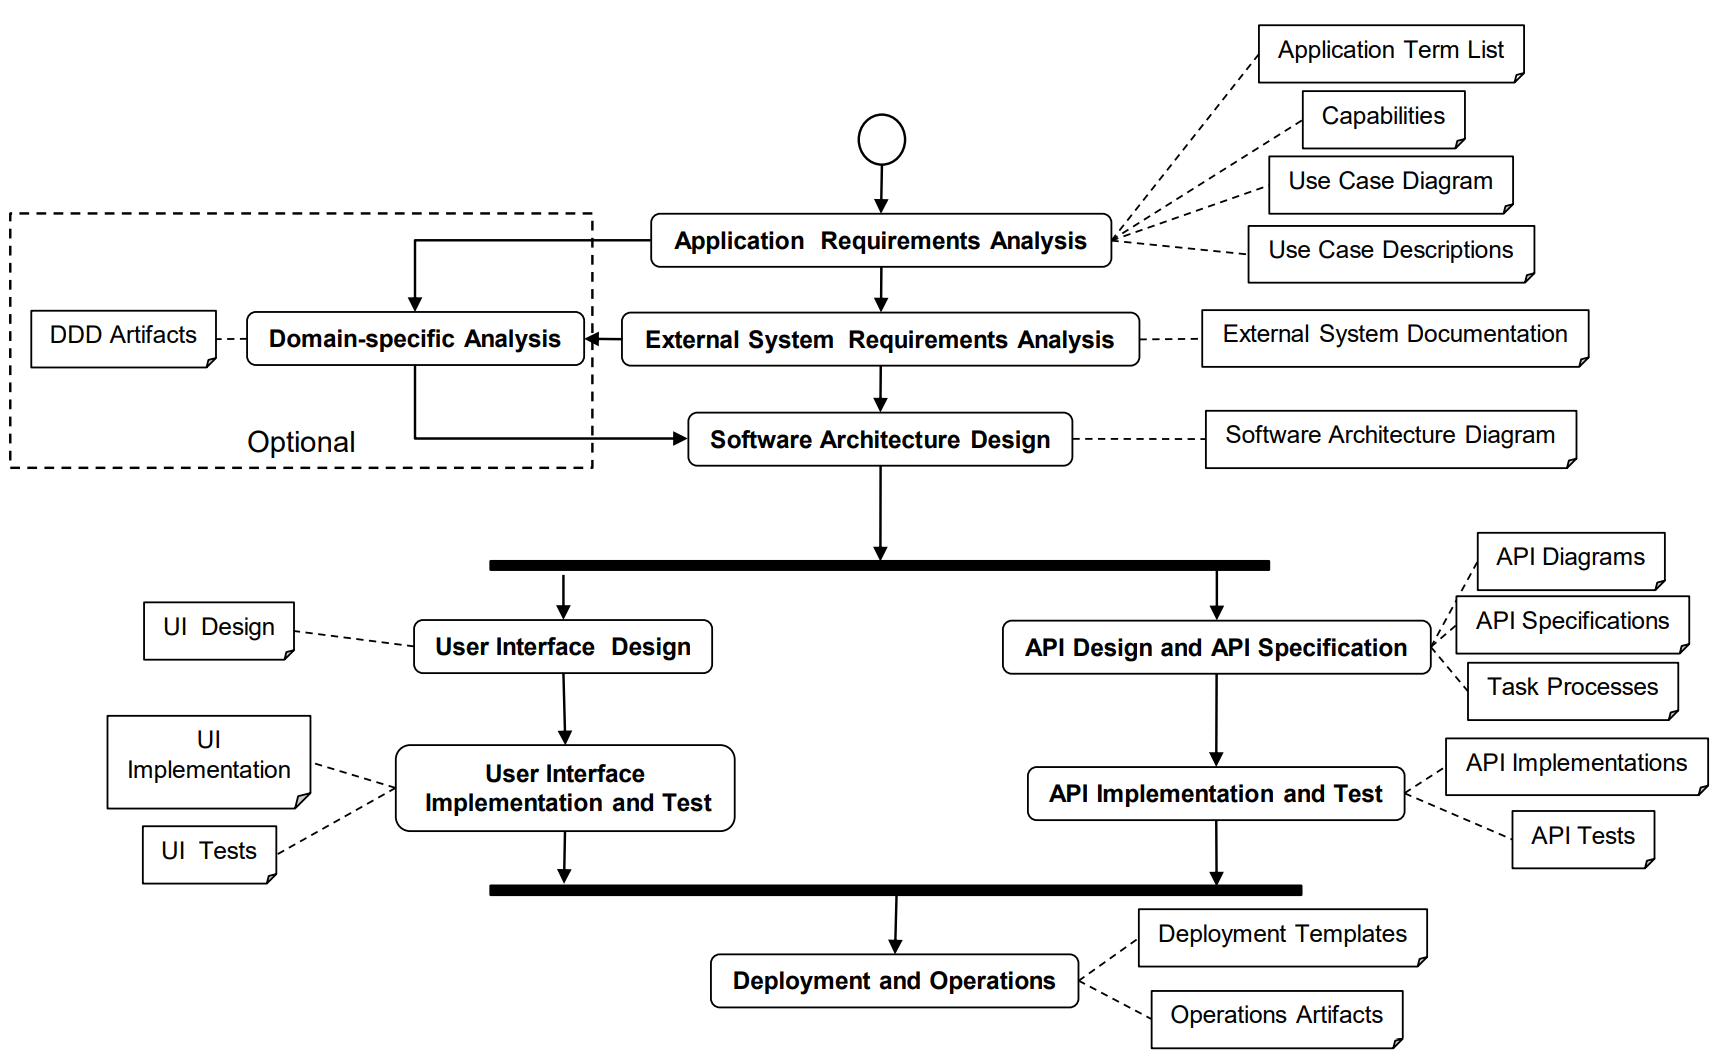
\includegraphics[width=\textwidth]{figures/ume_approach.png}
	\caption{Unified Microservice Engineering Approach \cite{CM-W-OVW}}
	\label{fig:ume_approach}
\end{figure}

\begin{figure}[h]
	\centering
	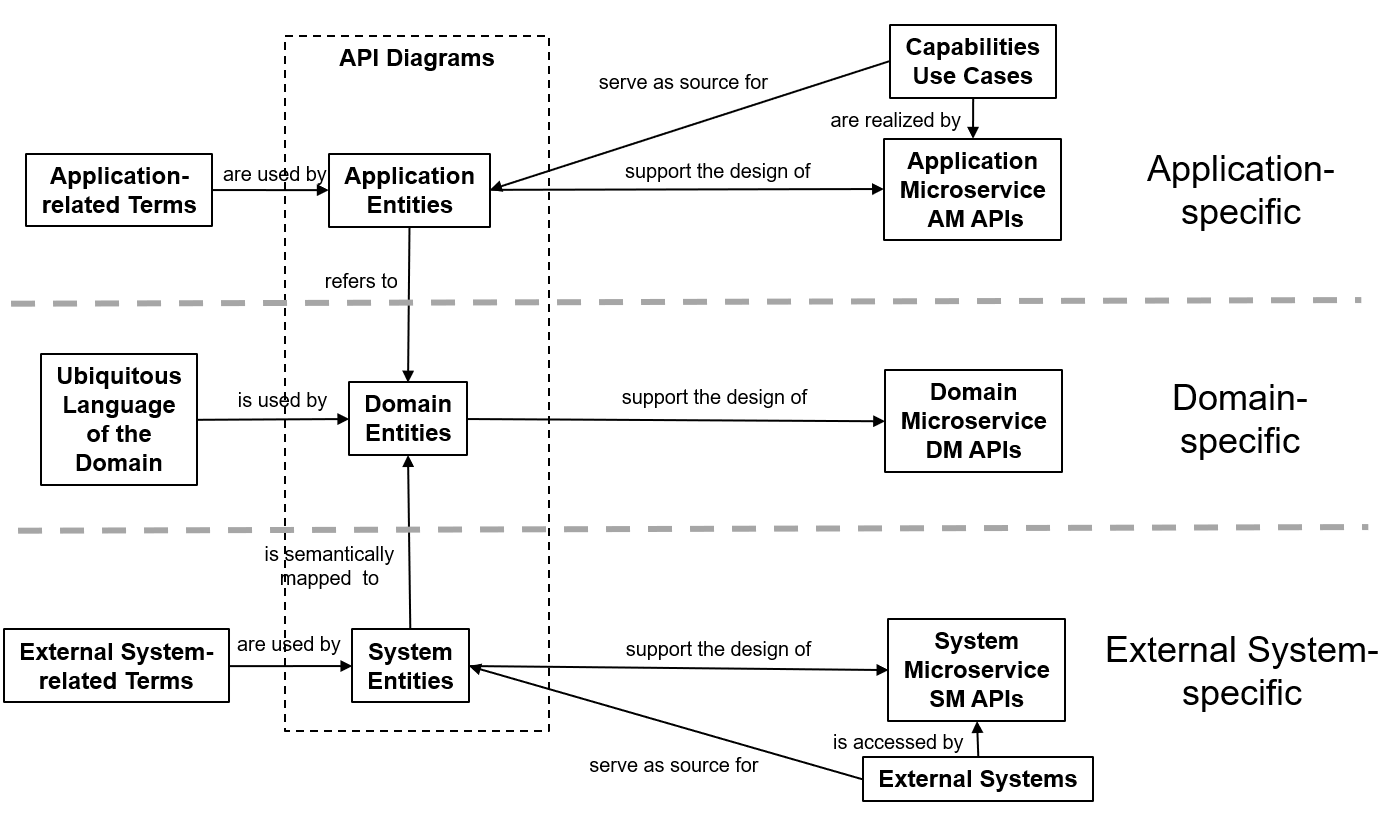
\includegraphics[width=\textwidth]{figures/ume_approach_api_design.png}
	\caption{UME Approach - API Design \cite{CM-W-DES}}
	\label{fig:ume_approach_api_design}
\end{figure}

% \begin{figure}[h]
% 	\centering
% 	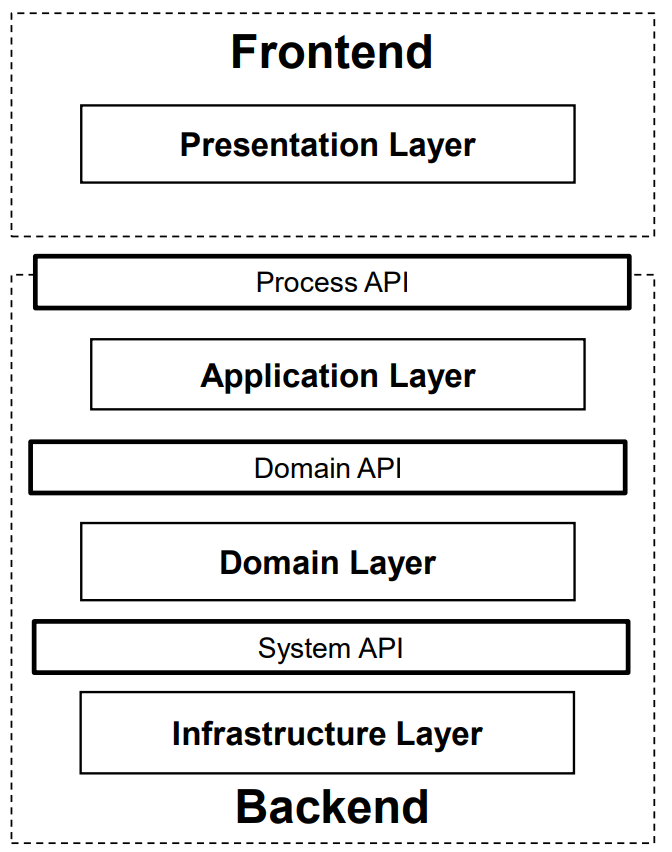
\includegraphics[width=\textwidth]{figures/ume_approach_layers.png}
% 	\caption{UME Approach - Architecture Layers}
% 	\label{fig:ume_approach_layers}
% \end{figure}

% \begin{figure}[h]
% 	\centering
% 	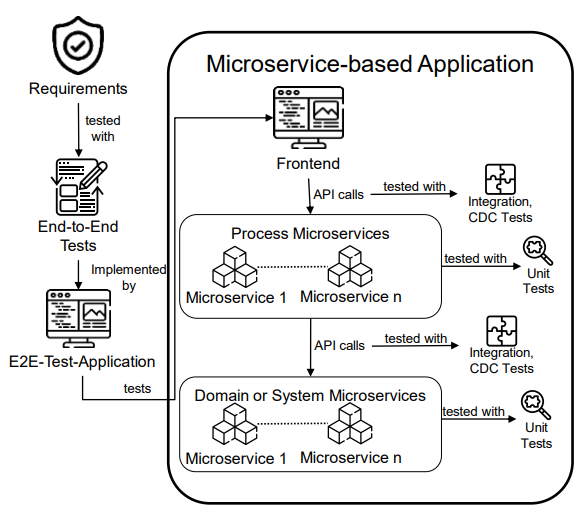
\includegraphics[width=\textwidth]{figures/ume_approach_test_concept.png}
% 	\caption{UME Approach - Test Concept}
% 	\label{fig:ume_approach_test_concept}
% \end{figure}

% \begin{figure}[h]
% 	\centering
% 	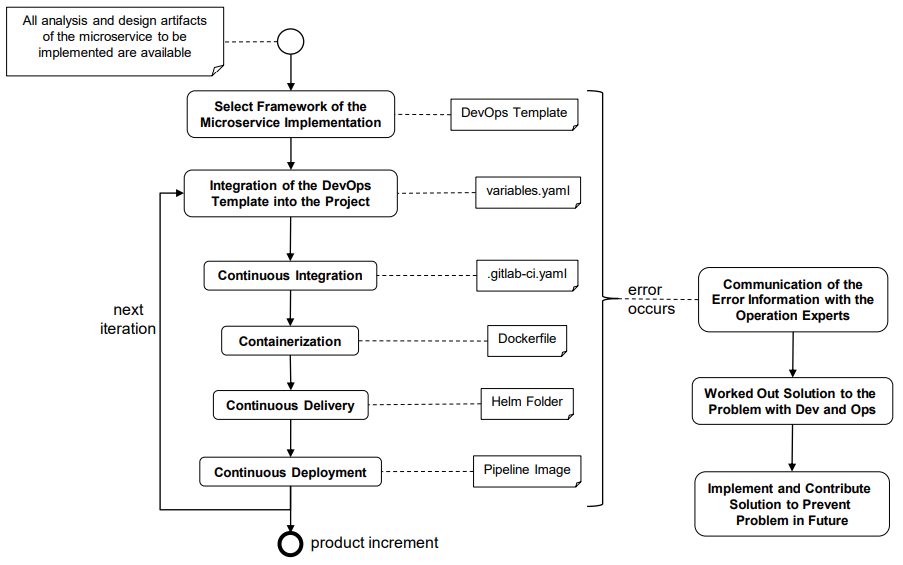
\includegraphics[width=\textwidth]{figures/ume_approach_deployment_operations.png}
% 	\caption{UME Approach - Deployment and Operations}
% 	\label{fig:ume_approach_deployment_operations}
% \end{figure}

% \begin{figure}[h]
% 	\centering
% 	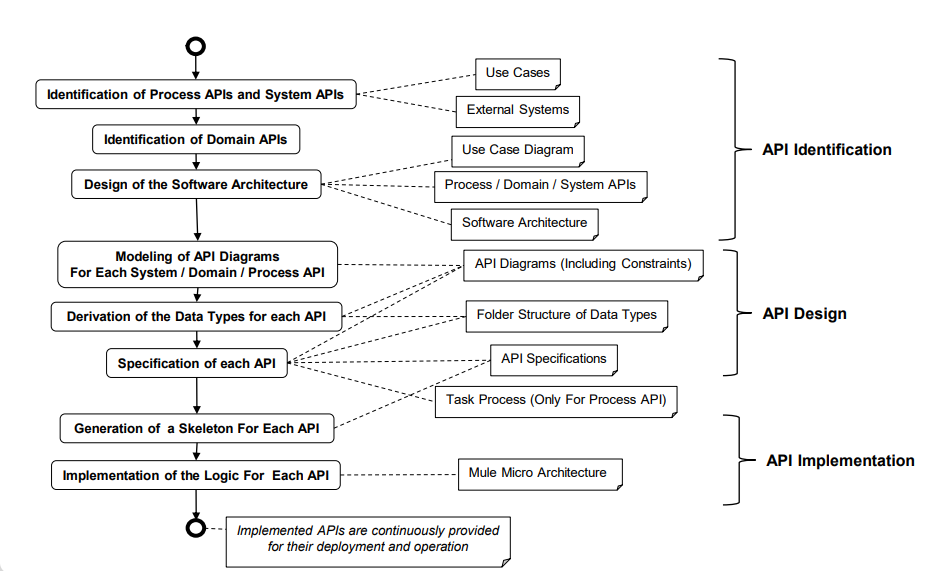
\includegraphics[width=\textwidth]{figures/ume_approach_api_related_actions.png}
% 	\caption{UME Approach - API related Actions}
% 	\label{fig:ume_approach_api_related_actions}
% \end{figure}

% TODO:
% - Software Architecture and System Architecture Diagram
% - Entities and API Design diagram ... also needs more explanation
% - API Diagram to API spec maybe with diagram but might be too much

The Unified Microservice Engineering (UME) approach is a software engineering
process developed by C\&M for the development of applications based on microservices.
An overview of the whole approach can be seen in Figure \ref{fig:ume_approach}.
It is based on two different approaches CMEng and MuleEng,
which were previously developed by C\&M.

% TODO: maybe something about CMEng and MuleEng?

The UME approach consists of four phases: Analysis, Design, Implementation and Test,
and Deployment and Operation. The approach can optionally be extended with domain-driven aspects.

The analysis phase starts with the Application Requirements Analysis
which analyzes and describes the requirements of the application that is to be developed.
This consists of creating an Application Term List which specificies the meaning
of application related terms for all involved parties. The Application Term List
is not a ubiquitous language as it is used in domain-driven design (DDD) because it
may span multiple different domains. Contrary, the ubiquitous language of DDD is always
specific to a single domain. Using the terms from the Application Term List,
capabilities and use cases are defined for the application. 
For each capability a separate use case diagram is created.
The use cases from each use case diagram are further specified in use case descriptions.
Optionally, the Application Requirements Analysis may be extended with additional artifacts
like a business vision and goals or an application sketch.
The standard analysis phase of the UME approach is concluded with the External System Requirements Analysis.
This analysis focues on specifying the requirements for external systems which will be used
by the application. Examples for such external systems are databases, enterprise applications,
and business services. The results of this analysis are documented in the External System Documentation.
In the case that the UME approach is extended with domain-driven aspects,
the analysis phase consists of an additional step: the Domain-specific Analysis.
This step encapsulates the standard DDD and its artifacts like ubiquitous languages
and domain models. % TODO: rewrite The addition of domain-driven aspects is useful when
% the application has to interact with services which may be used by multiple applications.
% In this case, the DDD Artifacts are used to construct Domain APIs which provide a layer
% of abstraction.

% TODO: Grafik für die verschiedenen API Schichten
% FIXME: are these still the right terms for the APIs
After the analysis phase comes the design phase which starts with the Software Architecture Design.
The software architecture of the application consists of Process, System, optional Domain, and Experience APIs.
The Process APIs are derived from use cases and directly provide the functionality set forth
by the use cases. There is a one-to-one mapping between methods of the Process APIs and the use cases.
System APIs are designed to integrated external systems into the application.
The optional Domain APIs provide domain-specific logic as a layer of abstraction
on top of the System APIs. Lastly, the Experience APIs
bridge the gap between the Process APIs which provide the logical functionality needed by
the application and its user interfaces. Different user interfaces may require
different forms of communication or data formats. For this reason, Experience APIs
are used as a layer of abstraction above the Process APIs with one Experience API
per user interface.
Note that during this design step, no specifications for the different APIs are created.
Instead the Software Architecture Design considers each API as a separate service
and constructs an architecture on how to arrange these services.
This is documented in a SystemPlusSoftware Architecture Diagram which is a type of UML
diagram developed by C\&M. % TODO: Explain SPS % A SystemPlusSoftware Architecture Diagram combines
% the physical and logical view of a system into a single diagram by combining
% UML Deployment Diagrams
After the design of the Software Architecture, the UME approach splits into two processes.
One for the user interfaces and one for the APIs.
Firstly, the APIs are designed and specifications are written for them.
The design of the API starts by creating API diagrams which model the entities relevant
for an API and their relationships to other APIs. Each type of API has a separate
type of API diagram and entities. There are Process API diagrams for Process APIs,
Domain API diagrams for Domain APIs, and System API diagrams for System APIs.
These diagrams consist, respectively, out of Process Entities, Domain Entities,
and System Entities. The relation between these entities, APIs and analysis artifacts
can be seen in Figure \ref{fig:ume_approach_api_design}.

Following the design of both the user interfaces and APIs,
the implementation and test phase starts in which all the APIs and user interfaces
are implemented according to their design. To ensure their correctness,
tests are also created. These tests consist of unit tests, integration tests and end-to-end tests.
Unit tests are written to ensure the correctness of single functions.
Integration tests then combine multiple functions together to test a complete API or user interface.
Finally, end-to-end tests verify the correctness of the whole application.
After the implementation and test phase, the two separate processes for the user interfaces
and APIs merge into a single process again. This starts the last phase: deployment and operations.
For the deployment of APIs and user interfaces, so called DevOps Templates are used
which can be reused across different projects. Configurable DevOps Templates reduce the complexity
of deployments because a certain variant of a deployment, like deploying a Go microservice
to a Kubernetes with Helm, only has to be created once and can then be reused with
the right configuration changes for other deployments.

\section{Monitoring in the DevOps Cycle}

% TODO: Do

As Ebert et al. \cite{EG+16} note, the research into DevOps is primarily concerned with
building and deploying software. But as the name implies, DevOps is also concerned with the
operation of software.

% TODO: Connection operation and observability

\begin{quote}
\textit{``Although researchers have focused considerably on build and deployment,
DevOps also impacts infrastructure operations'', \cite{EG+16}}
\end{quote}

\section{Integrating Monitoring into the Unified Microservice Engineering Approach}

% TODO: Do

Monitoring is a part of observability and as such should also be considered in DevOps processes.

% TODO: Business metrics and technical metrics

\begin{figure}[h]
	\centering
	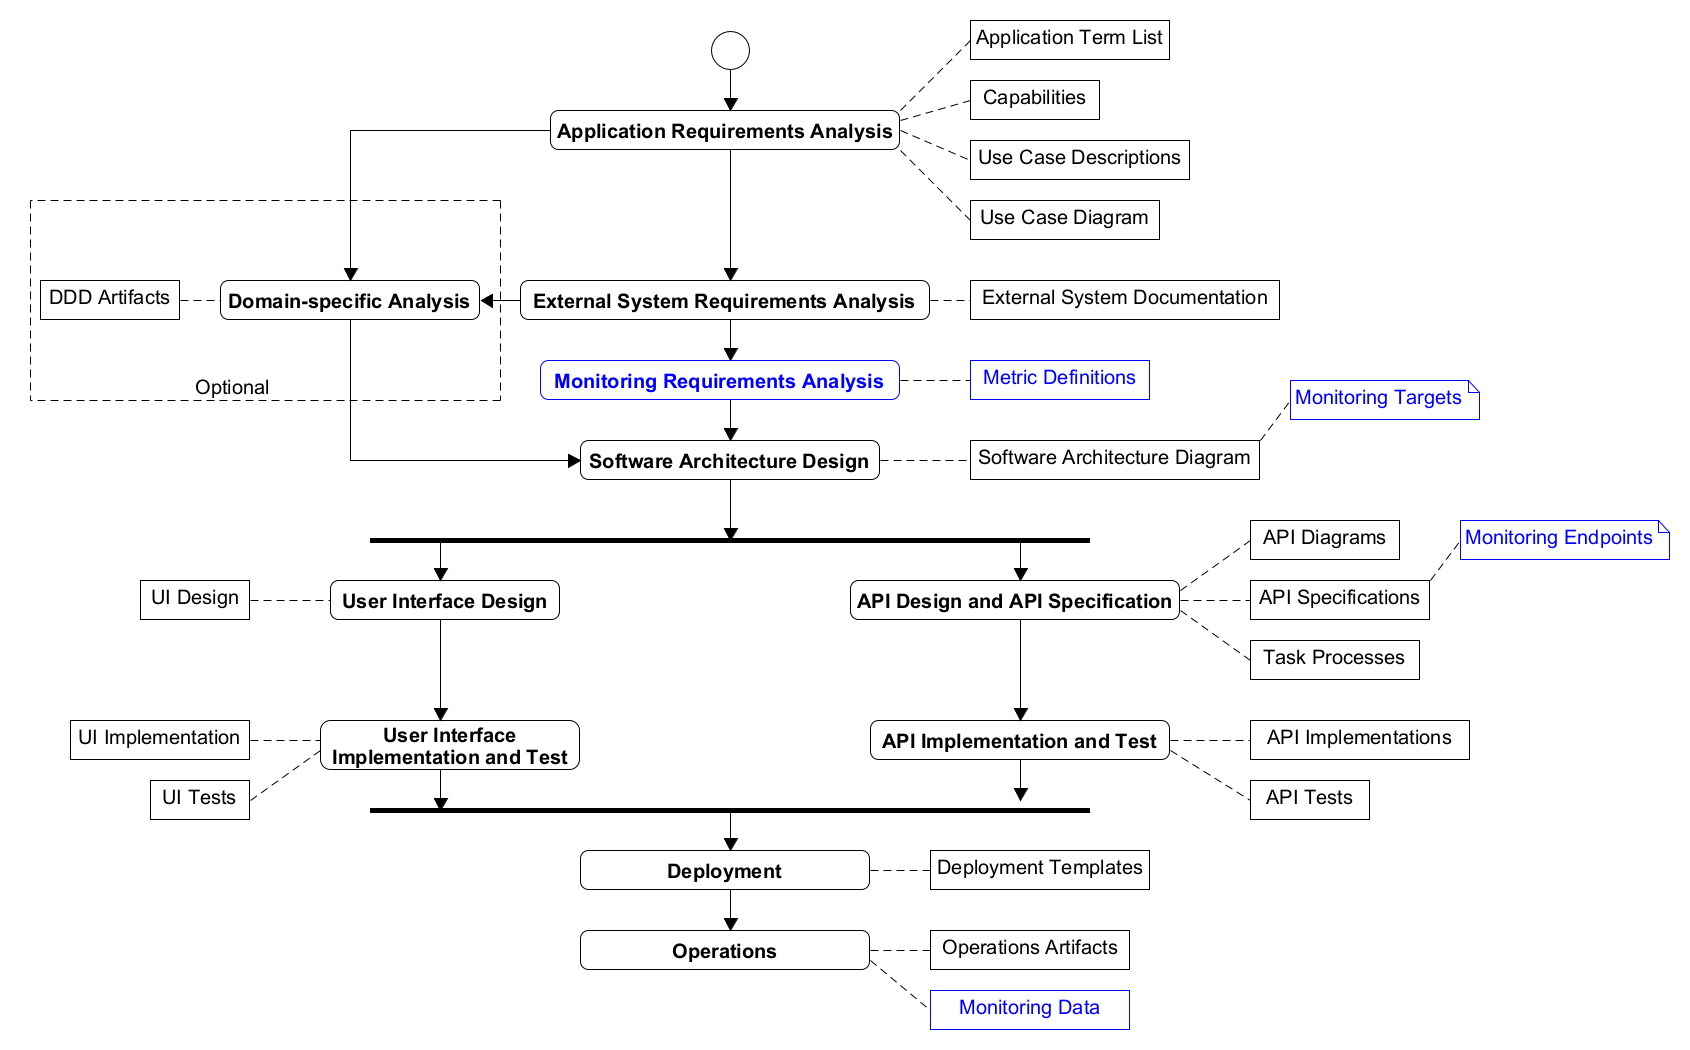
\includegraphics[width=\textwidth]{figures/ume_approach_extended.png}
	\caption{Extended Unified Microservice Approach}
	\label{fig:ume_approach_extended}
\end{figure}